\documentclass[class=scrreprt]{standalone}

\usepackage{amssymb}
\usepackage{bm}
\usepackage{pgfplots}
\pgfplotsset{compat=newest}
\usepgfplotslibrary{groupplots}

\KOMAoptions{fontsize=9pt}


  \begin{document}
  \begin{tikzpicture}
\draw[white](0,0) rectangle (12,11.5);
             \begin{scope}[xshift=3.5cm, yshift=8cm]
                 \node[] at (2.5,1.25)
                     {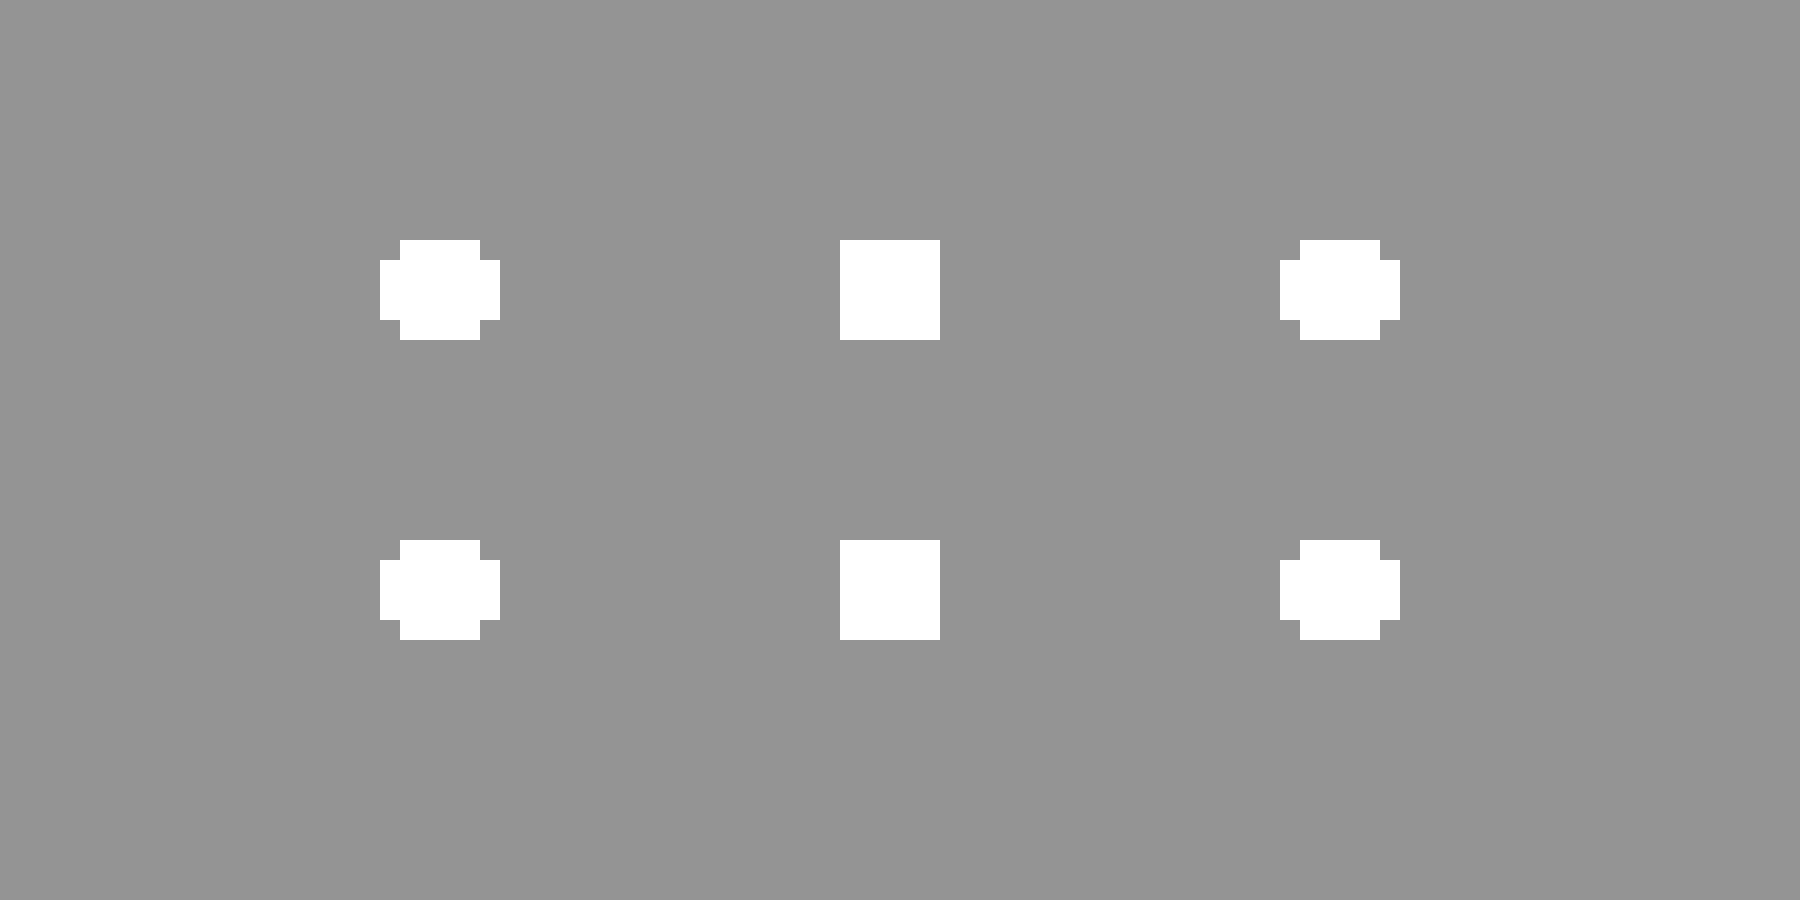
\includegraphics[width=5cm]{Figure_3/Input.png}};
                 \draw[step=0.0555555cm,black!75!white,very thin,shift={(0,0)}] (0,0)  grid(5,2.5);
                 \draw[black, thick] (0,0) rectangle(5,2.5);
                
                 % Bearings
                 \draw[black] (4.75,-0.25) -- (5,0) -- (5.25,-0.25)--  cycle;
                 \draw[black] (4.75,-0.5) -- (5.25,-0.5);
                 \draw[black] (4.75,-0.6)--(4.85,-0.5);
                 \draw[black] (4.85,-0.6)--(4.95,-0.5);
                 \draw[black] (4.95,-0.6)--(5.05,-0.5);
                 \draw[black] (5.05,-0.6)--(5.15,-0.5);
                 \draw[black] (5.15,-0.6)--(5.25,-0.5);
                 \draw[black] (5.125,-0.375) circle(0.125);
                 \draw[black] (4.875,-0.375) circle(0.125);
                
                 % Left bearings
                 \draw[black] (-0.25,0)--(-0.25,2.5);
                 \draw[black] (-0.35,0)--(-0.25,0.1);
                 \draw[black] (-0.35,0.1)--(-0.25,0.2);
                 \draw[black] (-0.35,0.2)--(-0.25,0.3);
                 \draw[black] (-0.35,0.3)--(-0.25,0.4);
                 \draw[black] (-0.35,0.4)--(-0.25,0.5);
                 \draw[black] (-0.35,0.5)--(-0.25,0.6);
                 \draw[black] (-0.35,0.6)--(-0.25,0.7);
                 \draw[black] (-0.35,0.7)--(-0.25,0.8);
                 \draw[black] (-0.35,0.8)--(-0.25,0.9);
                 \draw[black] (-0.35,0.9)--(-0.25,1.0);
                 \draw[black] (-0.35,1.0)--(-0.25,1.1);
                 \draw[black] (-0.35,1.1)--(-0.25,1.2);
                 \draw[black] (-0.35,1.2)--(-0.25,1.3);
                 \draw[black] (-0.35,1.3)--(-0.25,1.4);
                 \draw[black] (-0.35,1.4)--(-0.25,1.5);
                 \draw[black] (-0.35,1.5)--(-0.25,1.6);
                 \draw[black] (-0.35,1.6)--(-0.25,1.7);
                 \draw[black] (-0.35,1.7)--(-0.25,1.8);
                 \draw[black] (-0.35,1.8)--(-0.25,1.9);
                 \draw[black] (-0.35,1.9)--(-0.25,2.0);
                 \draw[black] (-0.35,2.0)--(-0.25,2.1);
                 \draw[black] (-0.35,2.1)--(-0.25,2.2);
                 \draw[black] (-0.35,2.2)--(-0.25,2.3);
                 \draw[black] (-0.35,2.3)--(-0.25,2.4);
                 \draw[black] (-0.35,2.4)--(-0.25,2.5);
                
                 \draw[black] (-0.125,0.125) circle(0.125);
                 \draw[black] (-0.125,0.375) circle(0.125);
                 \draw[black] (-0.125,0.625) circle(0.125);
                 \draw[black] (-0.125,0.875) circle(0.125);
                 \draw[black] (-0.125,1.125) circle(0.125);
                 \draw[black] (-0.125,1.375) circle(0.125);
                 \draw[black] (-0.125,1.625) circle(0.125);
                 \draw[black] (-0.125,1.875) circle(0.125);
                 \draw[black] (-0.125,2.125) circle(0.125);
                 \draw[black] (-0.125,2.375) circle(0.125);
                
                 % arrows
                 \draw[blue, thick] (-0.125,2.125)--(0,2)--(0,2.5)--(0.5,2.5)--(0.375,2.375);
                 \draw[blue, thick] (0.125,2.125)--(0,2);
                 \draw[blue, thick] (0.375,2.625)--(0.5,2.5);
                 \draw[red, thick] (0,3.25) -- (0,2.5);
                 \draw[red, thick] (-0.25,2.75)--(0,2.5)--(0.25,2.75);
                
                 % Label
                 \draw[red] (0,3) node[right] { $F$};
                 \draw[blue] (0,1.9) node[right] {$\bm{y}$};
                 \draw[blue] (0.375,2.25) node[right] { $\bm{x}$};
                
                
                 \node[black] at (0,-0.25) {\textbf{A}};
                
                
             \end{scope}
             \begin{scope}[xshift=0.5cm, yshift=4.5cm]
                 \node[] at (2.5,1.25)
                     {
\includegraphics[width=5cm]{Figure_3/X_homo.png}};
                 \draw[black, thick] (0,0) rectangle(5,2.5);% Bearings
                 \draw[black] (4.75,-0.25) -- (5,0) -- (5.25,-0.25)--  cycle;
                 \draw[black] (4.75,-0.5) -- (5.25,-0.5);
                 \draw[black] (4.75,-0.6)--(4.85,-0.5);
                 \draw[black] (4.85,-0.6)--(4.95,-0.5);
                 \draw[black] (4.95,-0.6)--(5.05,-0.5);
                 \draw[black] (5.05,-0.6)--(5.15,-0.5);
                 \draw[black] (5.15,-0.6)--(5.25,-0.5);
                 \draw[black] (5.125,-0.375) circle(0.125);
                 \draw[black] (4.875,-0.375) circle(0.125);
                
                 % Left bearings
                 \draw[black] (-0.25,0)--(-0.25,2.5);
                 \draw[black] (-0.35,0)--(-0.25,0.1);
                 \draw[black] (-0.35,0.1)--(-0.25,0.2);
                 \draw[black] (-0.35,0.2)--(-0.25,0.3);
                 \draw[black] (-0.35,0.3)--(-0.25,0.4);
                 \draw[black] (-0.35,0.4)--(-0.25,0.5);
                 \draw[black] (-0.35,0.5)--(-0.25,0.6);
                 \draw[black] (-0.35,0.6)--(-0.25,0.7);
                 \draw[black] (-0.35,0.7)--(-0.25,0.8);
                 \draw[black] (-0.35,0.8)--(-0.25,0.9);
                 \draw[black] (-0.35,0.9)--(-0.25,1.0);
                 \draw[black] (-0.35,1.0)--(-0.25,1.1);
                 \draw[black] (-0.35,1.1)--(-0.25,1.2);
                 \draw[black] (-0.35,1.2)--(-0.25,1.3);
                 \draw[black] (-0.35,1.3)--(-0.25,1.4);
                 \draw[black] (-0.35,1.4)--(-0.25,1.5);
                 \draw[black] (-0.35,1.5)--(-0.25,1.6);
                 \draw[black] (-0.35,1.6)--(-0.25,1.7);
                 \draw[black] (-0.35,1.7)--(-0.25,1.8);
                 \draw[black] (-0.35,1.8)--(-0.25,1.9);
                 \draw[black] (-0.35,1.9)--(-0.25,2.0);
                 \draw[black] (-0.35,2.0)--(-0.25,2.1);
                 \draw[black] (-0.35,2.1)--(-0.25,2.2);
                 \draw[black] (-0.35,2.2)--(-0.25,2.3);
                 \draw[black] (-0.35,2.3)--(-0.25,2.4);
                 \draw[black] (-0.35,2.4)--(-0.25,2.5);
                
                 \draw[black] (-0.125,0.125) circle(0.125);
                 \draw[black] (-0.125,0.375) circle(0.125);
                 \draw[black] (-0.125,0.625) circle(0.125);
                 \draw[black] (-0.125,0.875) circle(0.125);
                 \draw[black] (-0.125,1.125) circle(0.125);
                 \draw[black] (-0.125,1.375) circle(0.125);
                 \draw[black] (-0.125,1.625) circle(0.125);
                 \draw[black] (-0.125,1.875) circle(0.125);
                 \draw[black] (-0.125,2.125) circle(0.125);
                 \draw[black] (-0.125,2.375) circle(0.125);
                 \node[black] at (0,-0.25) {\textbf{B}};
             \end{scope}
             \begin{scope}[xshift=6.5cm, yshift=4.5cm]
                 \node[] at (2.5,1.25)
                     {
\includegraphics[width=5cm]{Figure_3/X_rand.png}};
                 \draw[black, thick] (0,0) rectangle(5,2.5);% Bearings
                 \draw[black] (4.75,-0.25) -- (5,0) -- (5.25,-0.25)--  cycle;
                 \draw[black] (4.75,-0.5) -- (5.25,-0.5);
                 \draw[black] (4.75,-0.6)--(4.85,-0.5);
                 \draw[black] (4.85,-0.6)--(4.95,-0.5);
                 \draw[black] (4.95,-0.6)--(5.05,-0.5);
                 \draw[black] (5.05,-0.6)--(5.15,-0.5);
                 \draw[black] (5.15,-0.6)--(5.25,-0.5);
                 \draw[black] (5.125,-0.375) circle(0.125);
                 \draw[black] (4.875,-0.375) circle(0.125);
                
                 % Left bearings
                 \draw[black] (-0.25,0)--(-0.25,2.5);
                 \draw[black] (-0.35,0)--(-0.25,0.1);
                 \draw[black] (-0.35,0.1)--(-0.25,0.2);
                 \draw[black] (-0.35,0.2)--(-0.25,0.3);
                 \draw[black] (-0.35,0.3)--(-0.25,0.4);
                 \draw[black] (-0.35,0.4)--(-0.25,0.5);
                 \draw[black] (-0.35,0.5)--(-0.25,0.6);
                 \draw[black] (-0.35,0.6)--(-0.25,0.7);
                 \draw[black] (-0.35,0.7)--(-0.25,0.8);
                 \draw[black] (-0.35,0.8)--(-0.25,0.9);
                 \draw[black] (-0.35,0.9)--(-0.25,1.0);
                 \draw[black] (-0.35,1.0)--(-0.25,1.1);
                 \draw[black] (-0.35,1.1)--(-0.25,1.2);
                 \draw[black] (-0.35,1.2)--(-0.25,1.3);
                 \draw[black] (-0.35,1.3)--(-0.25,1.4);
                 \draw[black] (-0.35,1.4)--(-0.25,1.5);
                 \draw[black] (-0.35,1.5)--(-0.25,1.6);
                 \draw[black] (-0.35,1.6)--(-0.25,1.7);
                 \draw[black] (-0.35,1.7)--(-0.25,1.8);
                 \draw[black] (-0.35,1.8)--(-0.25,1.9);
                 \draw[black] (-0.35,1.9)--(-0.25,2.0);
                 \draw[black] (-0.35,2.0)--(-0.25,2.1);
                 \draw[black] (-0.35,2.1)--(-0.25,2.2);
                 \draw[black] (-0.35,2.2)--(-0.25,2.3);
                 \draw[black] (-0.35,2.3)--(-0.25,2.4);
                 \draw[black] (-0.35,2.4)--(-0.25,2.5);
                
                 \draw[black] (-0.125,0.125) circle(0.125);
                 \draw[black] (-0.125,0.375) circle(0.125);
                 \draw[black] (-0.125,0.625) circle(0.125);
                 \draw[black] (-0.125,0.875) circle(0.125);
                 \draw[black] (-0.125,1.125) circle(0.125);
                 \draw[black] (-0.125,1.375) circle(0.125);
                 \draw[black] (-0.125,1.625) circle(0.125);
                 \draw[black] (-0.125,1.875) circle(0.125);
                 \draw[black] (-0.125,2.125) circle(0.125);
                 \draw[black] (-0.125,2.375) circle(0.125);
                 \node[black] at (0,-0.25) {\textbf{C}};
             \end{scope}
             \begin{scope}[xshift=0.5cm, yshift=1cm]
                 \node[] at (2.5,1.25)
                     {
\includegraphics[width=5cm]{Figure_3/X_post.png}};
                 \draw[black, thick] (0,0) rectangle(5,2.5);% Bearings
                 \draw[black] (4.75,-0.25) -- (5,0) -- (5.25,-0.25)--  cycle;
                 \draw[black] (4.75,-0.5) -- (5.25,-0.5);
                 \draw[black] (4.75,-0.6)--(4.85,-0.5);
                 \draw[black] (4.85,-0.6)--(4.95,-0.5);
                 \draw[black] (4.95,-0.6)--(5.05,-0.5);
                 \draw[black] (5.05,-0.6)--(5.15,-0.5);
                 \draw[black] (5.15,-0.6)--(5.25,-0.5);
                 \draw[black] (5.125,-0.375) circle(0.125);
                 \draw[black] (4.875,-0.375) circle(0.125);
                
                 % Left bearings
                 \draw[black] (-0.25,0)--(-0.25,2.5);
                 \draw[black] (-0.35,0)--(-0.25,0.1);
                 \draw[black] (-0.35,0.1)--(-0.25,0.2);
                 \draw[black] (-0.35,0.2)--(-0.25,0.3);
                 \draw[black] (-0.35,0.3)--(-0.25,0.4);
                 \draw[black] (-0.35,0.4)--(-0.25,0.5);
                 \draw[black] (-0.35,0.5)--(-0.25,0.6);
                 \draw[black] (-0.35,0.6)--(-0.25,0.7);
                 \draw[black] (-0.35,0.7)--(-0.25,0.8);
                 \draw[black] (-0.35,0.8)--(-0.25,0.9);
                 \draw[black] (-0.35,0.9)--(-0.25,1.0);
                 \draw[black] (-0.35,1.0)--(-0.25,1.1);
                 \draw[black] (-0.35,1.1)--(-0.25,1.2);
                 \draw[black] (-0.35,1.2)--(-0.25,1.3);
                 \draw[black] (-0.35,1.3)--(-0.25,1.4);
                 \draw[black] (-0.35,1.4)--(-0.25,1.5);
                 \draw[black] (-0.35,1.5)--(-0.25,1.6);
                 \draw[black] (-0.35,1.6)--(-0.25,1.7);
                 \draw[black] (-0.35,1.7)--(-0.25,1.8);
                 \draw[black] (-0.35,1.8)--(-0.25,1.9);
                 \draw[black] (-0.35,1.9)--(-0.25,2.0);
                 \draw[black] (-0.35,2.0)--(-0.25,2.1);
                 \draw[black] (-0.35,2.1)--(-0.25,2.2);
                 \draw[black] (-0.35,2.2)--(-0.25,2.3);
                 \draw[black] (-0.35,2.3)--(-0.25,2.4);
                 \draw[black] (-0.35,2.4)--(-0.25,2.5);
                
                 \draw[black] (-0.125,0.125) circle(0.125);
                 \draw[black] (-0.125,0.375) circle(0.125);
                 \draw[black] (-0.125,0.625) circle(0.125);
                 \draw[black] (-0.125,0.875) circle(0.125);
                 \draw[black] (-0.125,1.125) circle(0.125);
                 \draw[black] (-0.125,1.375) circle(0.125);
                 \draw[black] (-0.125,1.625) circle(0.125);
                 \draw[black] (-0.125,1.875) circle(0.125);
                 \draw[black] (-0.125,2.125) circle(0.125);
                 \draw[black] (-0.125,2.375) circle(0.125);
                 \node[black] at (0,-0.25) {\textbf{D}};
             \end{scope}
             \begin{scope}[xshift=6.5cm, yshift=1cm]
                 \node[] at (2.5,1.25)
                     {
\includegraphics[width=5cm]{Figure_3/BO_result.png}};
                 \draw[black, thick] (0,0) rectangle(5,2.5);% Bearings
                 \draw[black] (4.75,-0.25) -- (5,0) -- (5.25,-0.25)--  cycle;
                 \draw[black] (4.75,-0.5) -- (5.25,-0.5);
                 \draw[black] (4.75,-0.6)--(4.85,-0.5);
                 \draw[black] (4.85,-0.6)--(4.95,-0.5);
                 \draw[black] (4.95,-0.6)--(5.05,-0.5);
                 \draw[black] (5.05,-0.6)--(5.15,-0.5);
                 \draw[black] (5.15,-0.6)--(5.25,-0.5);
                 \draw[black] (5.125,-0.375) circle(0.125);
                 \draw[black] (4.875,-0.375) circle(0.125);
                
                 % Left bearings
                 \draw[black] (-0.25,0)--(-0.25,2.5);
                 \draw[black] (-0.35,0)--(-0.25,0.1);
                 \draw[black] (-0.35,0.1)--(-0.25,0.2);
                 \draw[black] (-0.35,0.2)--(-0.25,0.3);
                 \draw[black] (-0.35,0.3)--(-0.25,0.4);
                 \draw[black] (-0.35,0.4)--(-0.25,0.5);
                 \draw[black] (-0.35,0.5)--(-0.25,0.6);
                 \draw[black] (-0.35,0.6)--(-0.25,0.7);
                 \draw[black] (-0.35,0.7)--(-0.25,0.8);
                 \draw[black] (-0.35,0.8)--(-0.25,0.9);
                 \draw[black] (-0.35,0.9)--(-0.25,1.0);
                 \draw[black] (-0.35,1.0)--(-0.25,1.1);
                 \draw[black] (-0.35,1.1)--(-0.25,1.2);
                 \draw[black] (-0.35,1.2)--(-0.25,1.3);
                 \draw[black] (-0.35,1.3)--(-0.25,1.4);
                 \draw[black] (-0.35,1.4)--(-0.25,1.5);
                 \draw[black] (-0.35,1.5)--(-0.25,1.6);
                 \draw[black] (-0.35,1.6)--(-0.25,1.7);
                 \draw[black] (-0.35,1.7)--(-0.25,1.8);
                 \draw[black] (-0.35,1.8)--(-0.25,1.9);
                 \draw[black] (-0.35,1.9)--(-0.25,2.0);
                 \draw[black] (-0.35,2.0)--(-0.25,2.1);
                 \draw[black] (-0.35,2.1)--(-0.25,2.2);
                 \draw[black] (-0.35,2.2)--(-0.25,2.3);
                 \draw[black] (-0.35,2.3)--(-0.25,2.4);
                 \draw[black] (-0.35,2.4)--(-0.25,2.5);
                
                 \draw[black] (-0.125,0.125) circle(0.125);
                 \draw[black] (-0.125,0.375) circle(0.125);
                 \draw[black] (-0.125,0.625) circle(0.125);
                 \draw[black] (-0.125,0.875) circle(0.125);
                 \draw[black] (-0.125,1.125) circle(0.125);
                 \draw[black] (-0.125,1.375) circle(0.125);
                 \draw[black] (-0.125,1.625) circle(0.125);
                 \draw[black] (-0.125,1.875) circle(0.125);
                 \draw[black] (-0.125,2.125) circle(0.125);
                 \draw[black] (-0.125,2.375) circle(0.125);
                 \node[black] at (0,-0.25) {\textbf{E}};
             \end{scope}
 \end{tikzpicture}
 \end{document}